\section*{Assignment 4.8}

Let $X_1, \ldots, X_n$ be a random sample of size $n$ from a continuous distribution with median $M$. Let
\begin{align*}
X_{\min} = \min_{1\leq i\leq n} X_i, \qquad X_{\max} = \max_{1\leq i\leq n}X_i.
\end{align*}
\begin{enumerate}
	\item Show that
	\begin{align*}
	P[X_{\min} \leq M \leq X_{\max}] = 1 - \left(\frac{1}{2} \right)^{n-1}.
	\end{align*}
	\item Suppose the sample data are arranged from smallest to largest, so that $X_1\leq X_2\leq \cdots \leq X_n$. Calculate 
	\begin{align*}
	P[X_{k+1} \leq M\leq X_{n-k}]
	\end{align*}
	for $k = 0, \ldots, \lfloor n/2\rfloor$.
\end{enumerate}
\textbf{\underline{Solution}.} By definition of median, 
\begin{align*}
P[X_i\leq M] = \frac{1}{2},
\end{align*}
for $i = 1, \ldots, n$.
\begin{enumerate}
	\item We know that
	\begin{align*}
	P[X_{\min} \leq M \leq X_{\max}] & = 1 - P[X_{\min} > M] - P[X_{\max} < M] \\
	& = 1 - 2\cdot \left(\frac{1}{2} \right)^n \\
	& = 1 - \left(\frac{1}{2} \right)^{n-1}.
	\end{align*}
	\item Suppose we have a set of random variables $Y_i$, where $i = 1, \ldots, n$, denoting the random variables before reordering. Then each $Y_i$ is a Bernoulli random variable, and
	\begin{align*}
	P[Y_i\leq M] = \frac{1}{2}.
	\end{align*}
	Therefore, denoting
	\begin{align*}
	S = \{Y_1, \ldots, Y_n \},
	\end{align*}
	we have
	\begin{align*}
	P[X_{k+1}\leq M\leq X_{n-k}] & = 1 - P[X_{k+1} > M] - P[X_{n-k} < M] \\
	P[X_{k+1} > M] & = \sum_{i=0}^k P\left[\left|\{Y_j\in S: Y_j \leq M \}\right| = i\right] \\
	& = \sum_{i=0}^k\binom{n}{i}\left(\frac{1}{2} \right)^n \\
	P[X_{n-k} < M] & = \sum_{i=0}^k P\left[\left|\{Y_j\in S: Y_j \geq M \}\right| = i\right] \\
	& = \sum_{i=0}^k \binom{n}{i} \left(\frac{1}{2} \right)^n.
	\end{align*}
	Therefore,
	\begin{align*}
	P[X_{k+1}\leq M\leq X_{n-k}] = 1 - \sum_{i=0}^k \binom{n}{i} \left(\frac{1}{2} \right)^{n-1}.
	\end{align*}
\end{enumerate}



\section*{Exercise 1.}

The mean diameter of a metal rod produced by a machine is supposed to be 2.30mm. If the mean is different from this value by more than 0.2mm, it should be reported and concerned. Suppose the diameter of the rod $X$ follows a normal distribution with mean $\mu$ and variance $\sigma^2$. A random sample of size $n = 16$ is tested with following data.
\begin{table}[H]
	\centering
	\begin{tabular}{cccc}
		2.55 & 2.11 & 2.76 & 2.19 \\
		2.94 & 2.41 & 2.27 & 1.98 \\
		2.72 & 2.26 & 2.65 & 2.68 \\
		2.15 & 2.33 & 2.32 & 1.88
	\end{tabular}
\end{table}
\begin{enumerate}
	\item Set up and perform a suitable hypothesis test procedure for the mean such that the test conclusion will have at most 5\% chance of being in error. \\
	\textbf{\underline{Solution}.} We test the hypotheses
	\begin{align*}
	H_0:\mu = 2.30, \qquad H_1: |\mu - 2.30| \geq 0.2.
	\end{align*}
	The test statistic is given by
	\begin{align*}
	T_{n-1} = \frac{\overline{X}-2.30}{S/\sqrt{n}}\quad\Rightarrow\quad t_{n-1} = 1.158,
	\end{align*}
	and critical value $t_{0.025, 15} = 2.131$. Therefore, we fail to reject $H_0$ at the significance level of 5\%.
	\item Find a confidence interval for $\mu$ and compare with the results from (1). \\
	\textbf{\underline{Solution}.} A two-sided 95\% confidence interval for $\mu$ is given by
	\begin{align*}
	\overline{X} \pm \frac{t_{0.025, 15} S}{\sqrt{n}}\quad\Rightarrow\quad \U{CI} = [2.227, 2.547].
	\end{align*}
	The null value 2.30 falls inside this confidence interval. Therefore, $H_0$ is not rejected, which is in accordance with the conclusion in (1).
	\item How large does the sample size should be to guarantee (1)? \\
	\textbf{\underline{Solution}.} We use the OC curve for two-sided T-test with $\alpha = 0.05$ and use the sample variance to estimate $\sigma^2$,
	\begin{align*}
	d = \frac{0.2}{S} \quad\Rightarrow\quad d \approx 0.66.
	\end{align*}
	\begin{figure}[H]
		\centering
		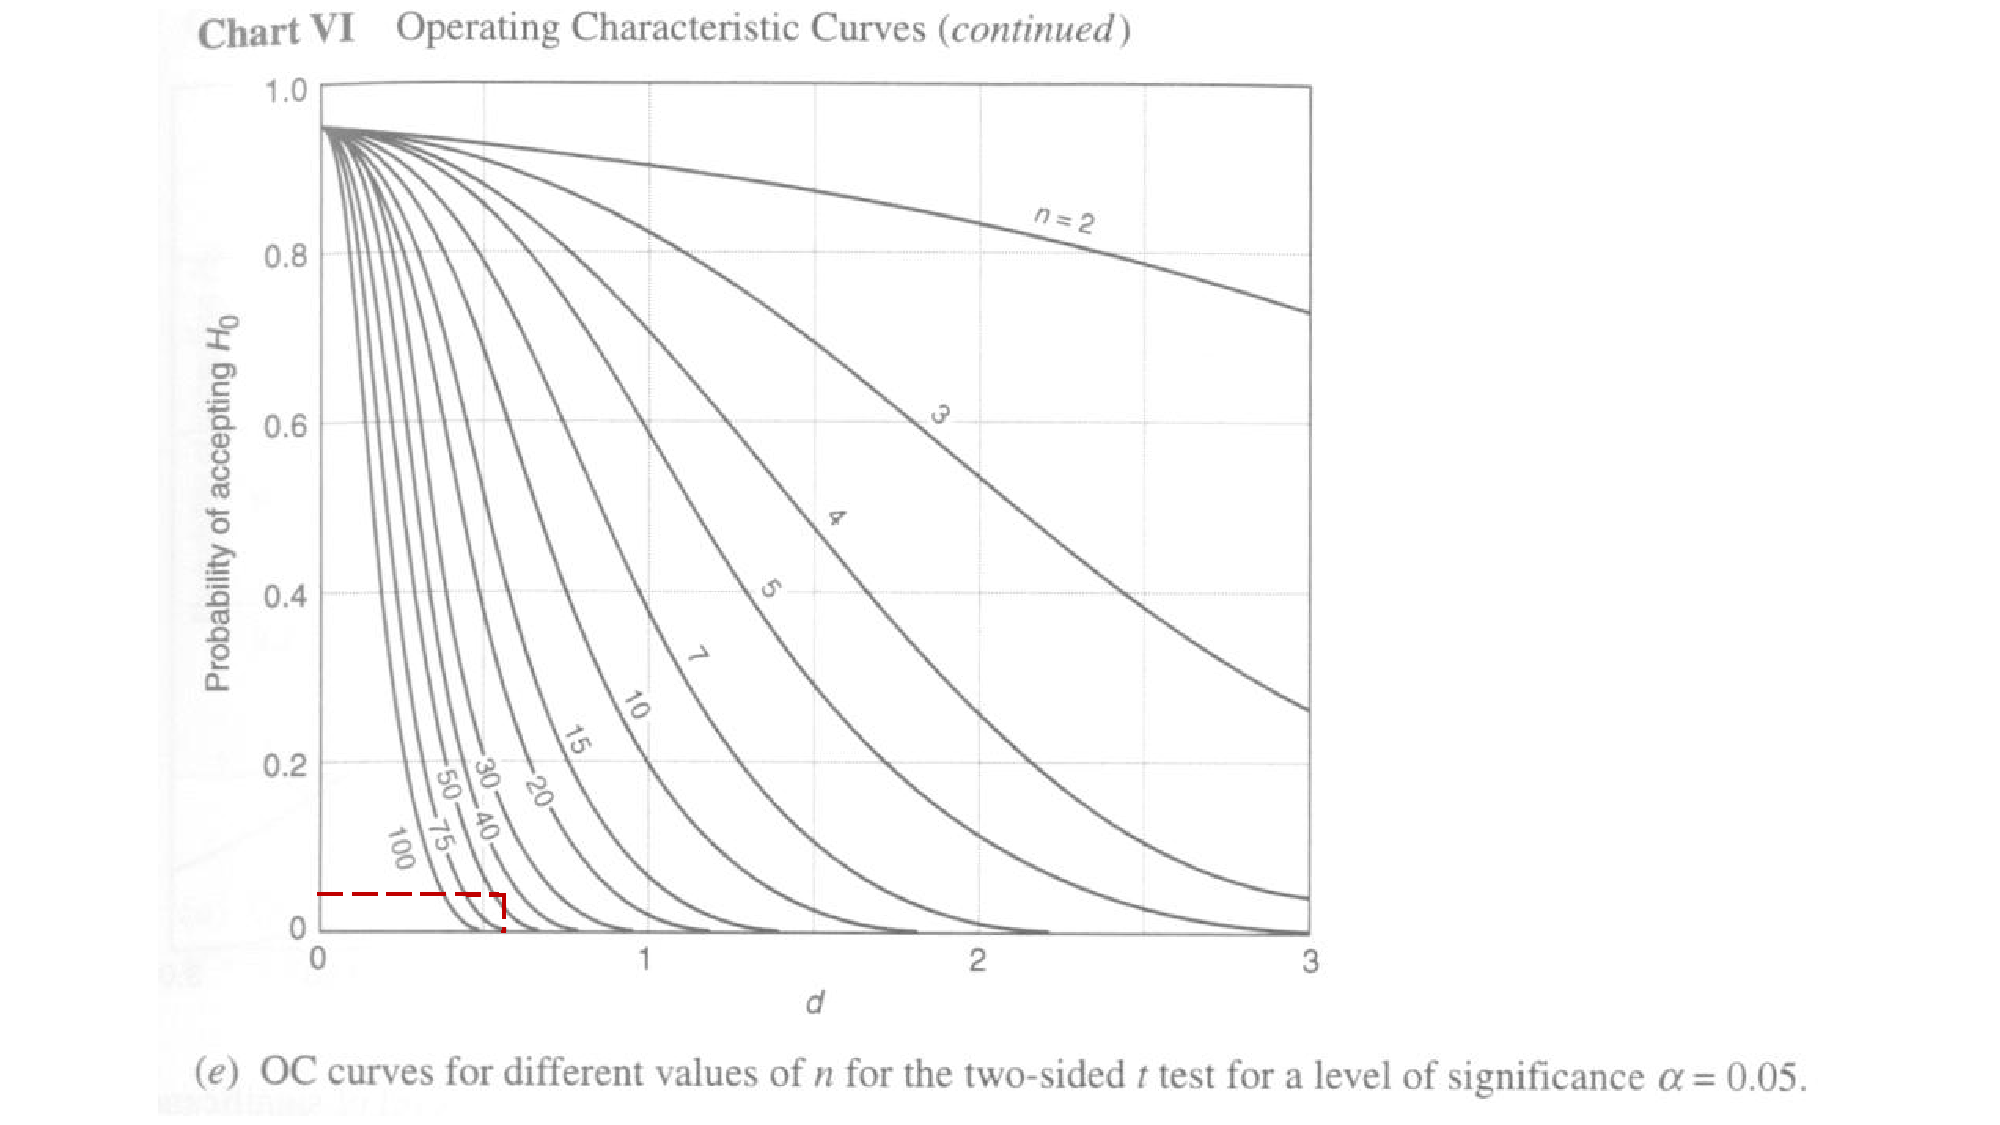
\includegraphics[width=\linewidth]{./images/s5fig1.pdf}
	\end{figure}
	We read from OC curve that $n\approx 47$ would be a sufficient sample size.
	\item If it is further required that the standard deviation of the normal distribution should be less than 0.5mm, set up and perform a suitable hypothesis test for the variance such that the test conclusion will have at most 5\% chance of being in error. \\
	\textbf{\underline{Solution}.} We test the hypothesis
	\begin{align*}
	H_0: \sigma \geq 0.5, \qquad H_1: \sigma < 0.5
	\end{align*}
	and obtain the test statistic
	\begin{align*}
	\chi_{n-1}^2 = \frac{(n-1)S^2}{0.5^2} \quad\Rightarrow\quad \chi_{n-1}^2 = 5.48,
	\end{align*}
	and critical value $\chi_{0.95, 15}^2 = 7.261$. Therefore, we reject $H_0$ at significance level $\alpha = 5\%$ and thus accept $H_1$.
	\item Find a confidence interval for $\sigma^2$ and compare with the results from (4). \\
	\textbf{\underline{Solution}.} A one-sided 95\% confidence interval for $\sigma^2$ is given by
	\begin{align*}
	\sigma^2 < \frac{(n-1)S^2}{\chi_{0.95, n-1}}\quad\Rightarrow\quad \sigma^2 < 0.026,
	\end{align*}
	and thus the null value $\sigma_0^2 = 0.25$ falls outside this interval. Therefore, $H_0$ is rejected, which is in accordance with the conclusion in (4).
	\item What the true value of $\sigma$ is necessary so that the test will have a power larger than 0.95? \\
	\textbf{\underline{Solution}.} We use the OC curve for one-sided Chi-squared test with $\alpha = 0.05$ and use the sample variance to estimate $\sigma^2$
	\begin{align*}
	\lambda = \frac{\sigma}{0.5} < 0.6\quad\Rightarrow\quad \sigma < 0.3.
	\end{align*}
	\begin{figure}[H]
		\centering
		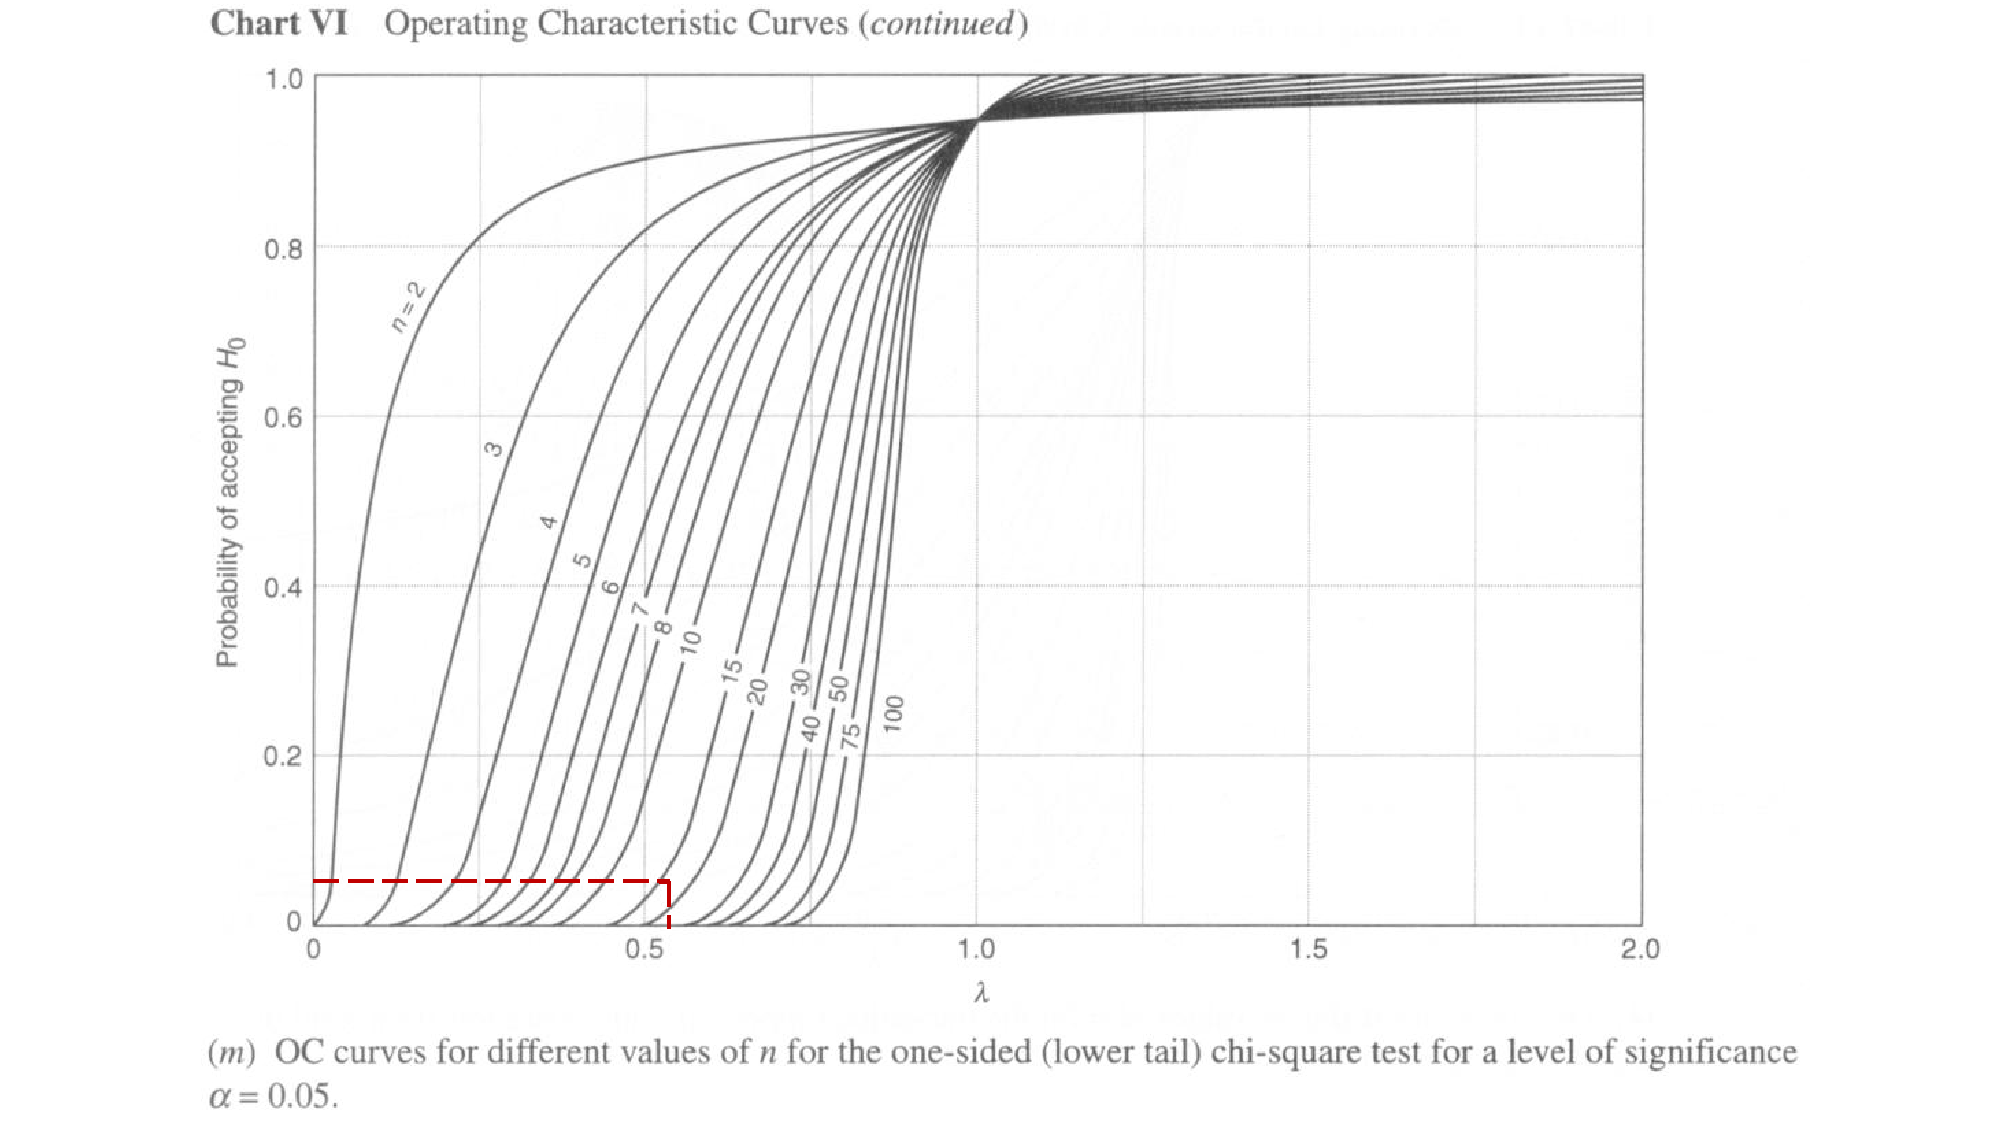
\includegraphics[width=\linewidth]{./images/s5fig2.pdf}
	\end{figure}
	\item Suppose we have no knowledge about the distribution, perform a sign test for the following hypothesis for the median $M$
	\begin{align*}
	H_0: M = 2.50
	\end{align*}
	with $\alpha = 0.05$. \\
	\textbf{\underline{Solution}.} We get the following table of signs.
	\begin{table}[H]
		\centering
		\begin{tabular}{cc|cc|cc|cc}
			\hline
			$X_i$ & Sign & $X_i$ & Sign & $X_i$ & Sign & $X_i$ & Sign \\
			\hline
			2.55 & + & 2.11 & - & 2.76 & + & 2.19 & - \\
			2.94 & + & 2.41 & - & 2.27 & - & 1.98 & - \\
			2.72 & + & 2.26 & - & 2.65 & + & 2.68 & + \\
			2.15 & - & 2 33 & - & 2.32 & - & 1.88 & - \\
			\hline
		\end{tabular}
	\end{table}
	Therefore, $q_+ = 6, q_- = 10, n' = q_+ + q_- = 16$. Since it is a two-tailed test, we have the p-value
	\begin{align*}
	p\U{-value} = 2\sum_{x=0}^{\min(q_+, q_-)} \binom{n'}{x} \frac{1}{2^n} = 0.454,
	\end{align*}
	with which we fail to reject $H_0$.
	\item Suppose we only know that the distribution of diameter is symmetric, perform a Wilcoxon signed rank test for the median $M$
	\begin{align*}
	H_0: M = 2.50
	\end{align*}
	with $\alpha = 0.05$. \\
	\textbf{\underline{Solution}.} We get the following table of signed ranks.
	\begin{table}[H]
		\centering
		\begin{tabular}{cc|cc|cc|cc}
			\hline
			$X_i$ & Rank & $X_i$ & Rank & $X_i$ & Rank & $X_i$ & Rank \\
			\hline
			2.55 & +1 & 2.68 & +5 & 2.26 & -9 & 2.11 & -13 \\
			2.41 & -2 & 2.32 & -6 & 2.76 & +10 & 2.94 & +14 \\
			2.65 & +3 & 2.72 & +7 & 2.19 & -11 & 1.98 & -15 \\
			2.33 & -4 & 2.27 & -8 & 2.15 & -12 & 1.88 & -16 \\
			\hline
		\end{tabular}
	\end{table}
	Then
	\begin{align*}
	W_+ = \sum_{R_i > 0} R_i\quad\Rightarrow\quad w_+ = 40, \qquad |W_-| = \sum_{R_i < 0} |R_i| \quad\Rightarrow\quad |w_-| = 96
	\end{align*}
	with $n' = n = 16$. Looking up the table for \underline{two-tailed} test with $\alpha=0.05$, we get a critical value of 29, which is smaller than $\min(W_+, |W_-|) = 40$. Therefore, we fail to reject $H_0$. Alternatively, we approximate the distribution of $|W_-|$ by a normal distribution with
	\begin{align*}
	\mu = \frac{n(n+1)}{4} = 68, \qquad \sigma = \sqrt{\frac{n(n+1)(2n+1)}{24}} = 19.34
	\end{align*}
	and normalize to obtain
	\begin{align*}
	z = \frac{|w_-| - \mu}{\sigma} = 1.45.
	\end{align*}
	We have the critical value $z_{0.025} = 1.96 > z$. Therefore, we fail to reject $H_0$.
	\begin{figure}[H]
		\centering
		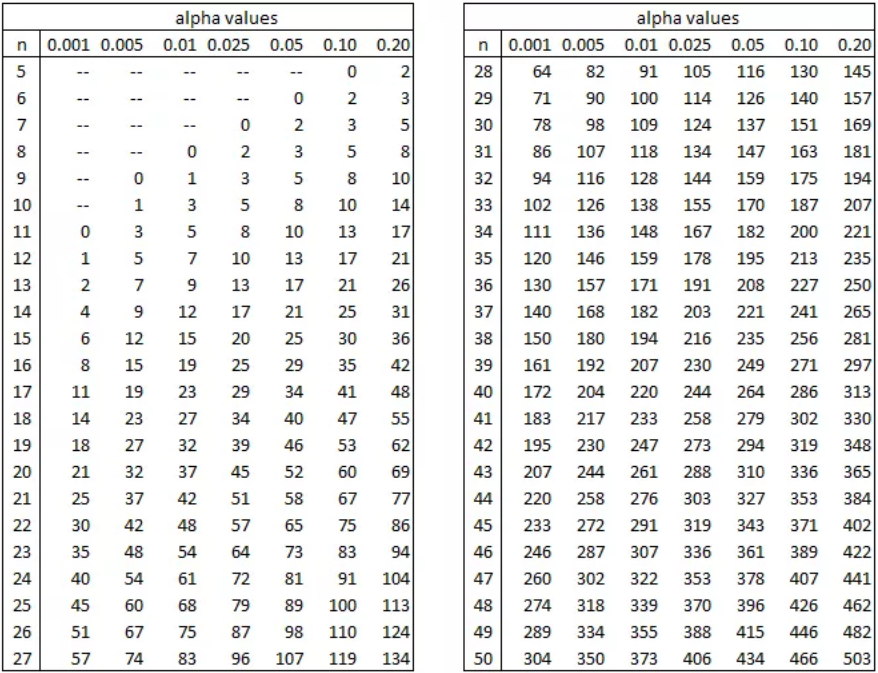
\includegraphics[width=14cm]{./images/s5fig3.png}
	\end{figure}
	\textbf{\underline{Note}.} The table above is for \underline{two-tailed} tests. We need to double the $\alpha$ in \underline{one-tailed} tests for table lookup, e.g., if $\alpha = 0.005$ is required, we use $\alpha = 0.01$ when looking up in the table.
	\item It is said that if the diameter falls in a range of $2.30\pm 0.40$mm, then the metal rod is of good quality. Perform the following test on proportion of good-quality rods that are produced by the machine.
	\begin{align*}
	H_0: p \leq 0.50,
	\end{align*}
	with $\alpha = 0.05$, where $p$ is the proportion of good-quality rods. \\
	\textbf{\underline{Solution}.} We have the estimate for proportion
	\begin{align*}
	\widehat{p} = \frac{\#\{X_i:X_i\in (1.90, 2.70) \}}{n} = 0.75.
	\end{align*}
	We have the statistic
	\begin{align*}
	Z = \frac{\widehat{p} - p_0}{\sqrt{p_0(1-p_0)/n}}\quad\Rightarrow\quad z = 2.0,
	\end{align*}
	and critical value $z_{\alpha} = 1.645 < z$. Therefore, we reject $H_0$ with at least 5\% level of significance.
	\item Another sample of 12 rods are tested. Perform a test comparing the proportions of good-quality rods of these two samples with $\alpha = 0.05$.
	\begin{table}[H]
		\centering
		\begin{tabular}{cccc}
			2.85 & 2.73 & 2.92 & 2.11 \\
			1.78 & 2.01 & 2.16 & 2.32 \\
			2.51 & 2.53 & 2.67 & 2.75
		\end{tabular}
	\end{table}
	\textbf{\underline{Solution}.} With the hypothesis
	\begin{align*}
	H_0: p_1 = p_2,
	\end{align*}
	we have the pooled proportion
	\begin{align*}
	\widehat{p} = \frac{n_1\widehat{p}_1 + n_2\widehat{p}_2}{n_1 + n_2} = 0.679,
	\end{align*}
	where $\widehat{p}_2 = 0.583$. We have the test statistic
	\begin{align*}
	Z = \frac{\widehat{p}_1 - \widehat{p}_2}{\sqrt{\widehat{p}(1-\widehat{p})\left(\dfrac{1}{n_1} + \dfrac{1}{n_2} \right)}} \quad\Rightarrow\quad z = 0.935
	\end{align*}
	and critical value $z_{\alpha/2} = 1.96 > z$. Therefore, we fail to reject $H_0$.\\
	\textbf{\underline{Note}.} You might argue that the sample sizes of questions (9) and (10) are not sufficient for hypothesis tests for proportions. They are presented simply for illustrative purpose.
	\item Perform a hypothesis test regarding the variances for the two samples with $\alpha = 0.05$.
	\begin{align*}
	H_0: \sigma_1^2 = \sigma_2^2
	\end{align*}
	\textbf{\underline{Solution}.} We calculate
	\begin{align*}
	S_1^2 & = \frac{1}{n_1-1}\sum_{i=1}^{n_1}(X_i^{(1)}-\overline{X}_1)^2\quad\Rightarrow\quad s_1^2 = 0.091  \\
	S_2^2 & = \frac{1}{n_2-1}\sum_{i=1}^{n_2}(X_i^{(2)}-\overline{X}_2)^2 \quad\Rightarrow\quad s_2^2 = 0.133,
	\end{align*}
	and thus the test statistics
	\begin{align*}
	F_{n_1-1,n_2-1} = \frac{S_1^2}{S_2^2}\ \Rightarrow\  f_{n_1-1,n_2-1} = 0.685, \qquad F_{n_2-1,n_1-1} = \frac{S_2^2}{S_1^2}\ \Rightarrow\  f_{n_2-1,n_1-1} = 1.460.
	\end{align*}
	The critical values are given by
	\begin{align*}
	f_{0.025, 15, 11} = 3.33, \qquad f_{0.025, 11, 15} = 3.01.
	\end{align*}
	Therefore, we fail to reject $H_0$.
\end{enumerate}
